
\subsubsection{Análisis para $R_{amort}$ en modo tensión, $V_{out} = 10 \si[per-mode=symbol]{\volt}$, $R_{L} = 10 \si[per-mode=symbol]{\ohm}$}

Se puede ver en la figura~\figref{fig:fig_power_supply_RAMORT_LOOP_Modo1} de ganancia de lazo para $R_{amort} = 0 \si[per-mode=symbol]{\ohm} $ que el margen de ganancia es $0.04 \si[per-mode=symbol]{\decibel} $ y el margen de fase es $0.09 \si[per-mode=symbol]{\degree} $ muy cercanas a la condición de oscilación  y en el gráfico de respuesta transitoria para $R_{amort} = 0 \si[per-mode=symbol]{\ohm} $, figura~\figref{fig:fig_power_supply_RAMORT_STEP_0_Modo1}, se ve como el sistema tiene una oscilación muy pequeña una vez que se alcanza la tensión del escalón y se mantiene hasta finalizar este, ya que no hay elemento disipativo, en cambio con $R_{amort} = 1 \si[per-mode=symbol]{\ohm} $, figura~\figref{fig:fig_power_supply_RAMORT_STEP_1_Modo1}, o $R_{amort} = 5 \si[per-mode=symbol]{\ohm} $, figura~\figref{fig:fig_power_supply_RAMORT_STEP_5_Modo1}, la respuesta transitoria ya no oscila, además se mejoran ampliamente los márgenes de fase y ganancia.

\vfill


% RAMORT MODO 1.

\clearpage

\begin{figure}[H] %htb
\begin{center}
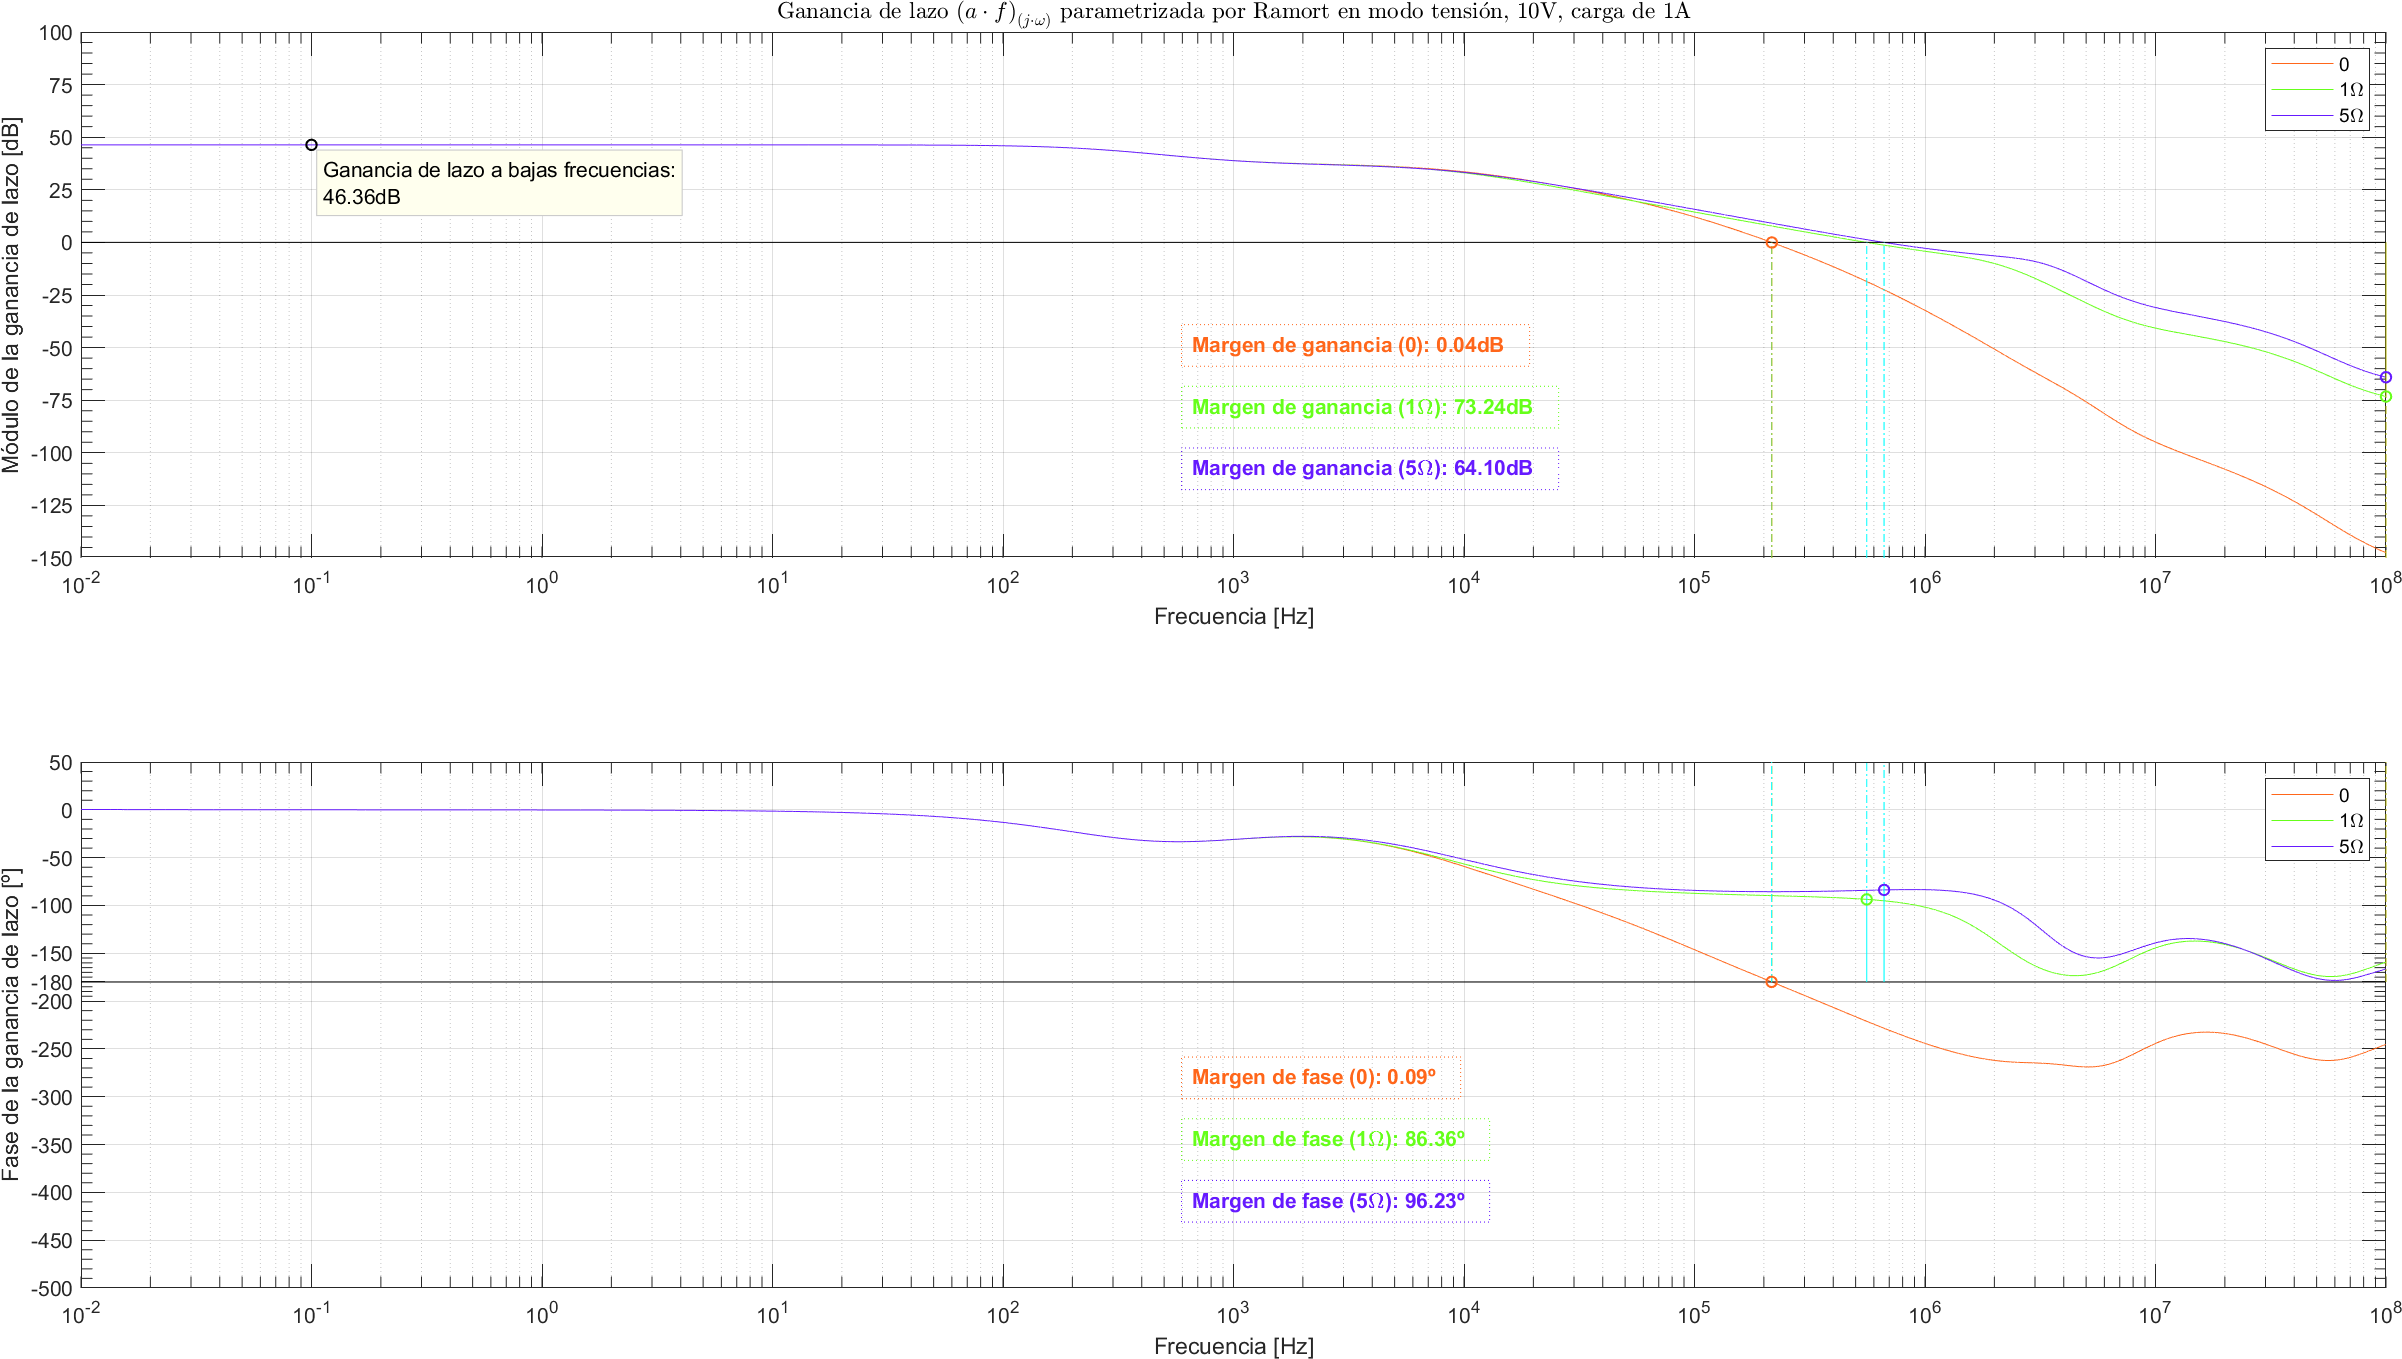
\includegraphics[width=1.1 \textwidth, angle=90]{./img/plots/loop/power_supply_RAMORT_LOOP_Modo1.png}
\caption{\label{fig:fig_power_supply_RAMORT_LOOP_Modo1}\footnotesize{Ganancia de lazo en modo tensión, $V_{out} = 10 \si[per-mode=symbol]{\volt}$, en función de la frecuencia parametrizada por $R_{amort}$.}}
\end{center}
\end{figure}


\clearpage

\begin{figure}[H] %htb
\begin{center}
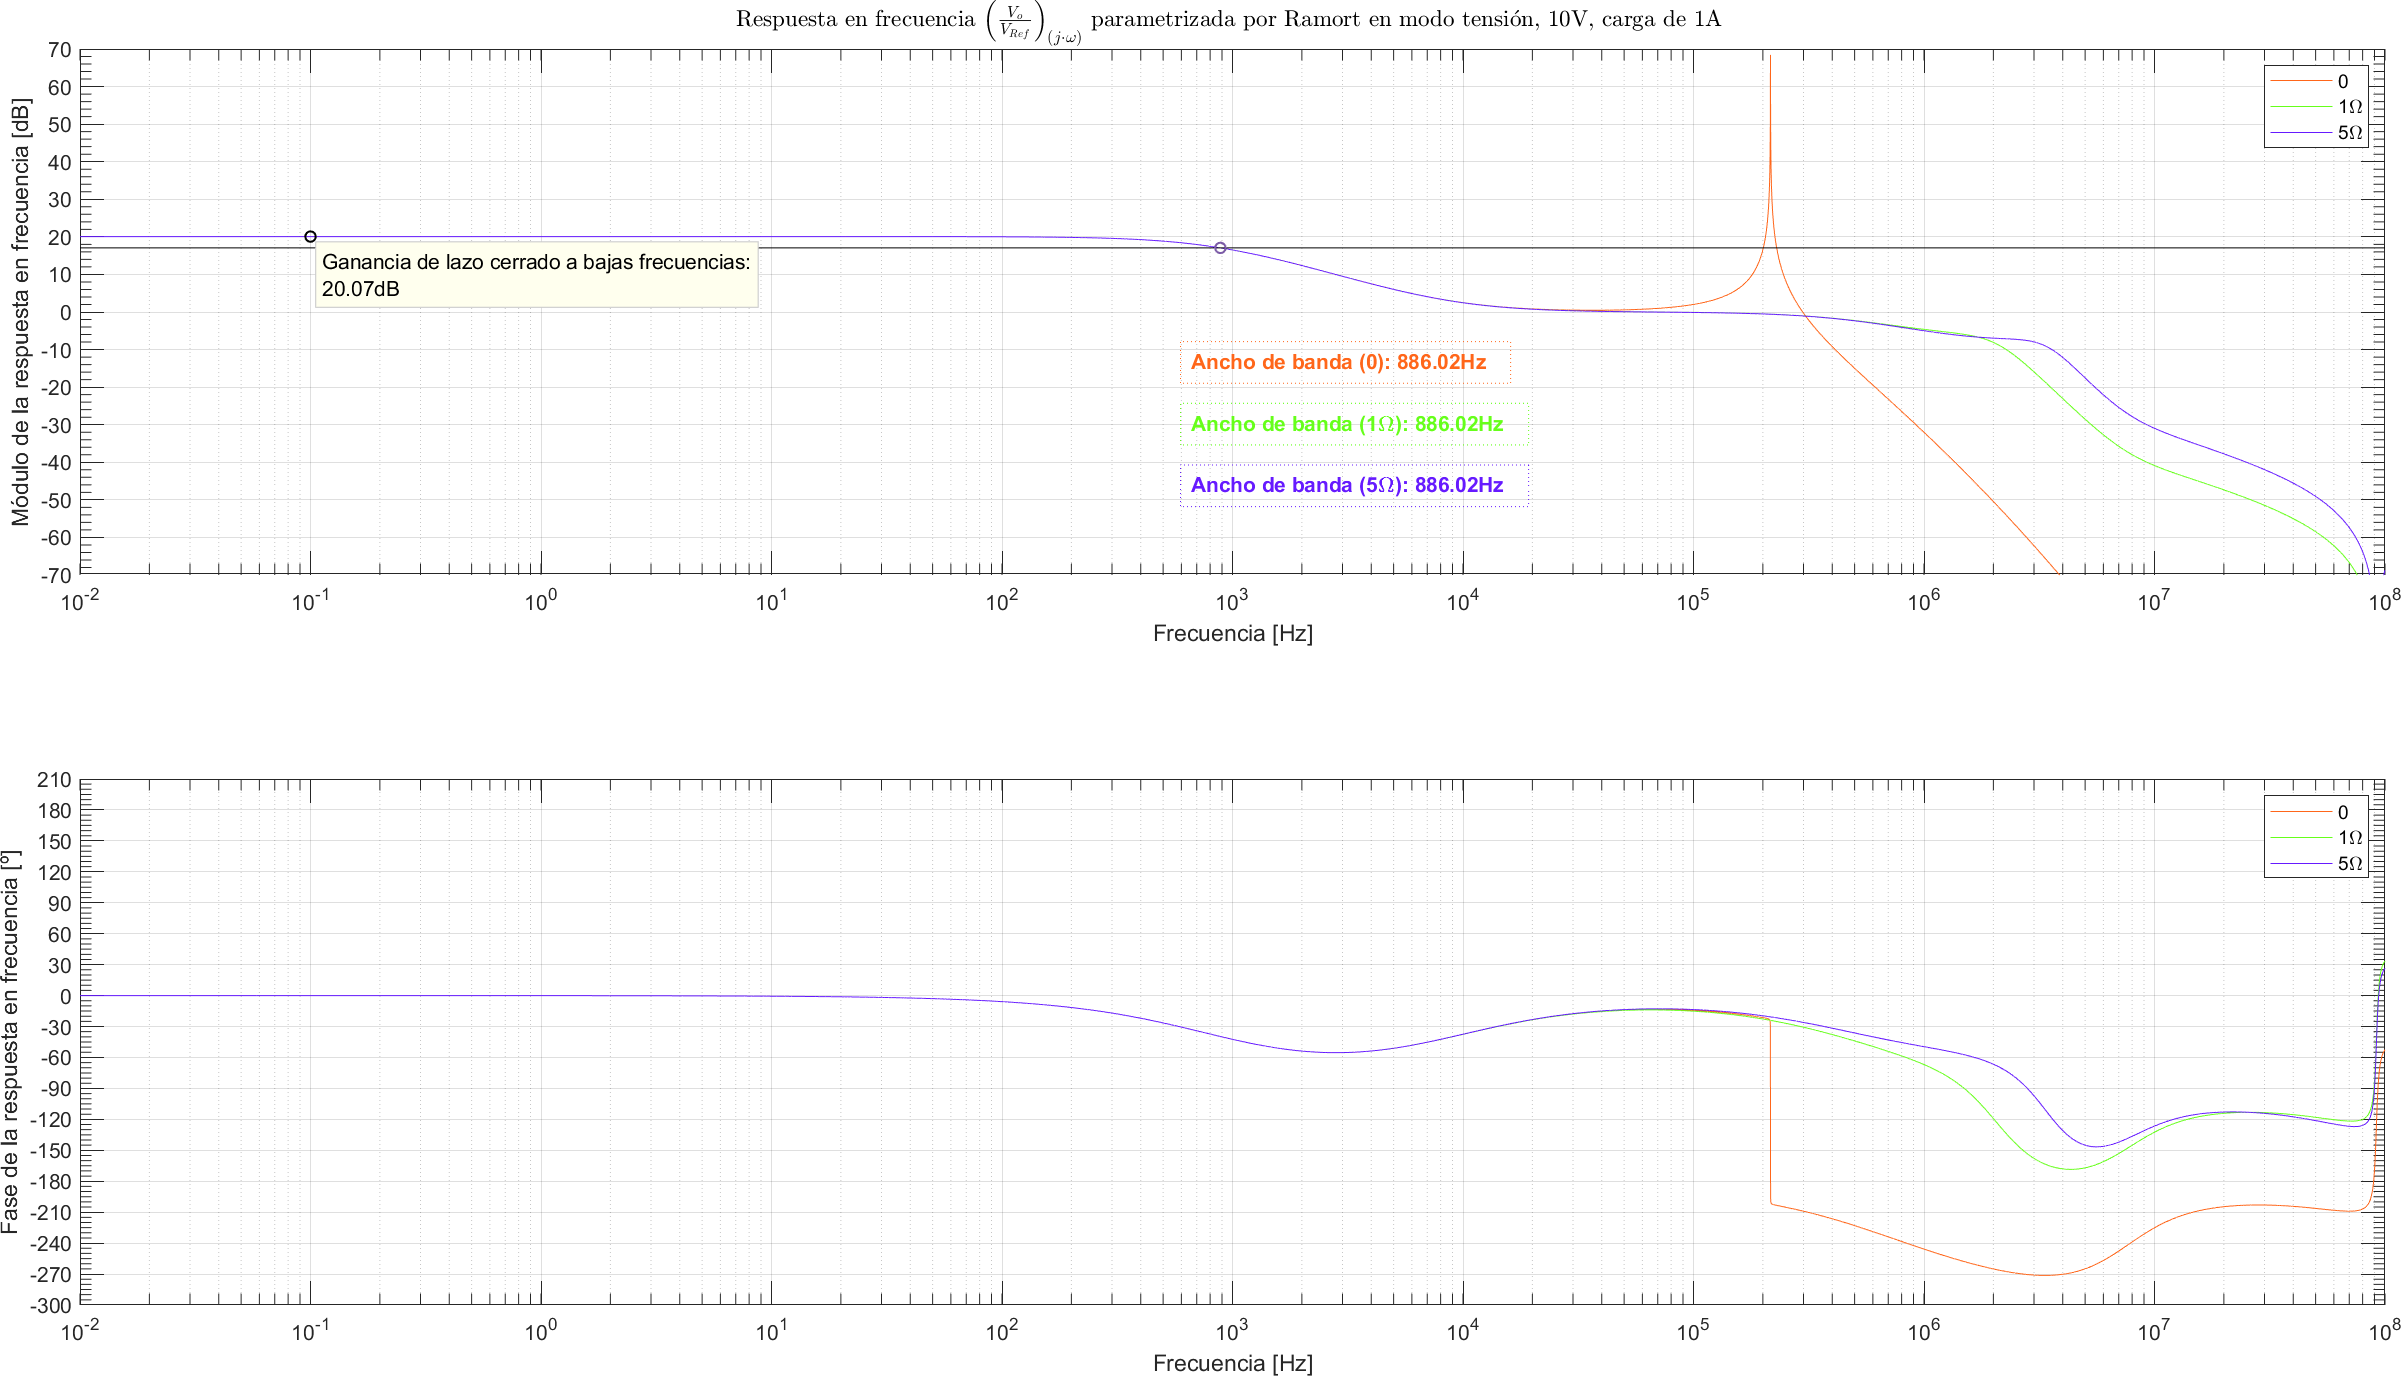
\includegraphics[width=1.1 \textwidth, angle=90]{./img/plots/rf/power_supply_RAMORT_RF_Modo1.png}
\caption{\label{fig:fig_power_supply_RAMORT_RF_Modo1}\footnotesize{Respuesta en frecuencia en modo tensión, $V_{out} = 10 \si[per-mode=symbol]{\volt}$, en función de la frecuencia parametrizada por $R_{amort}$.}}
\end{center}
\end{figure}

\clearpage

\begin{figure}[H] %htb
\begin{center}
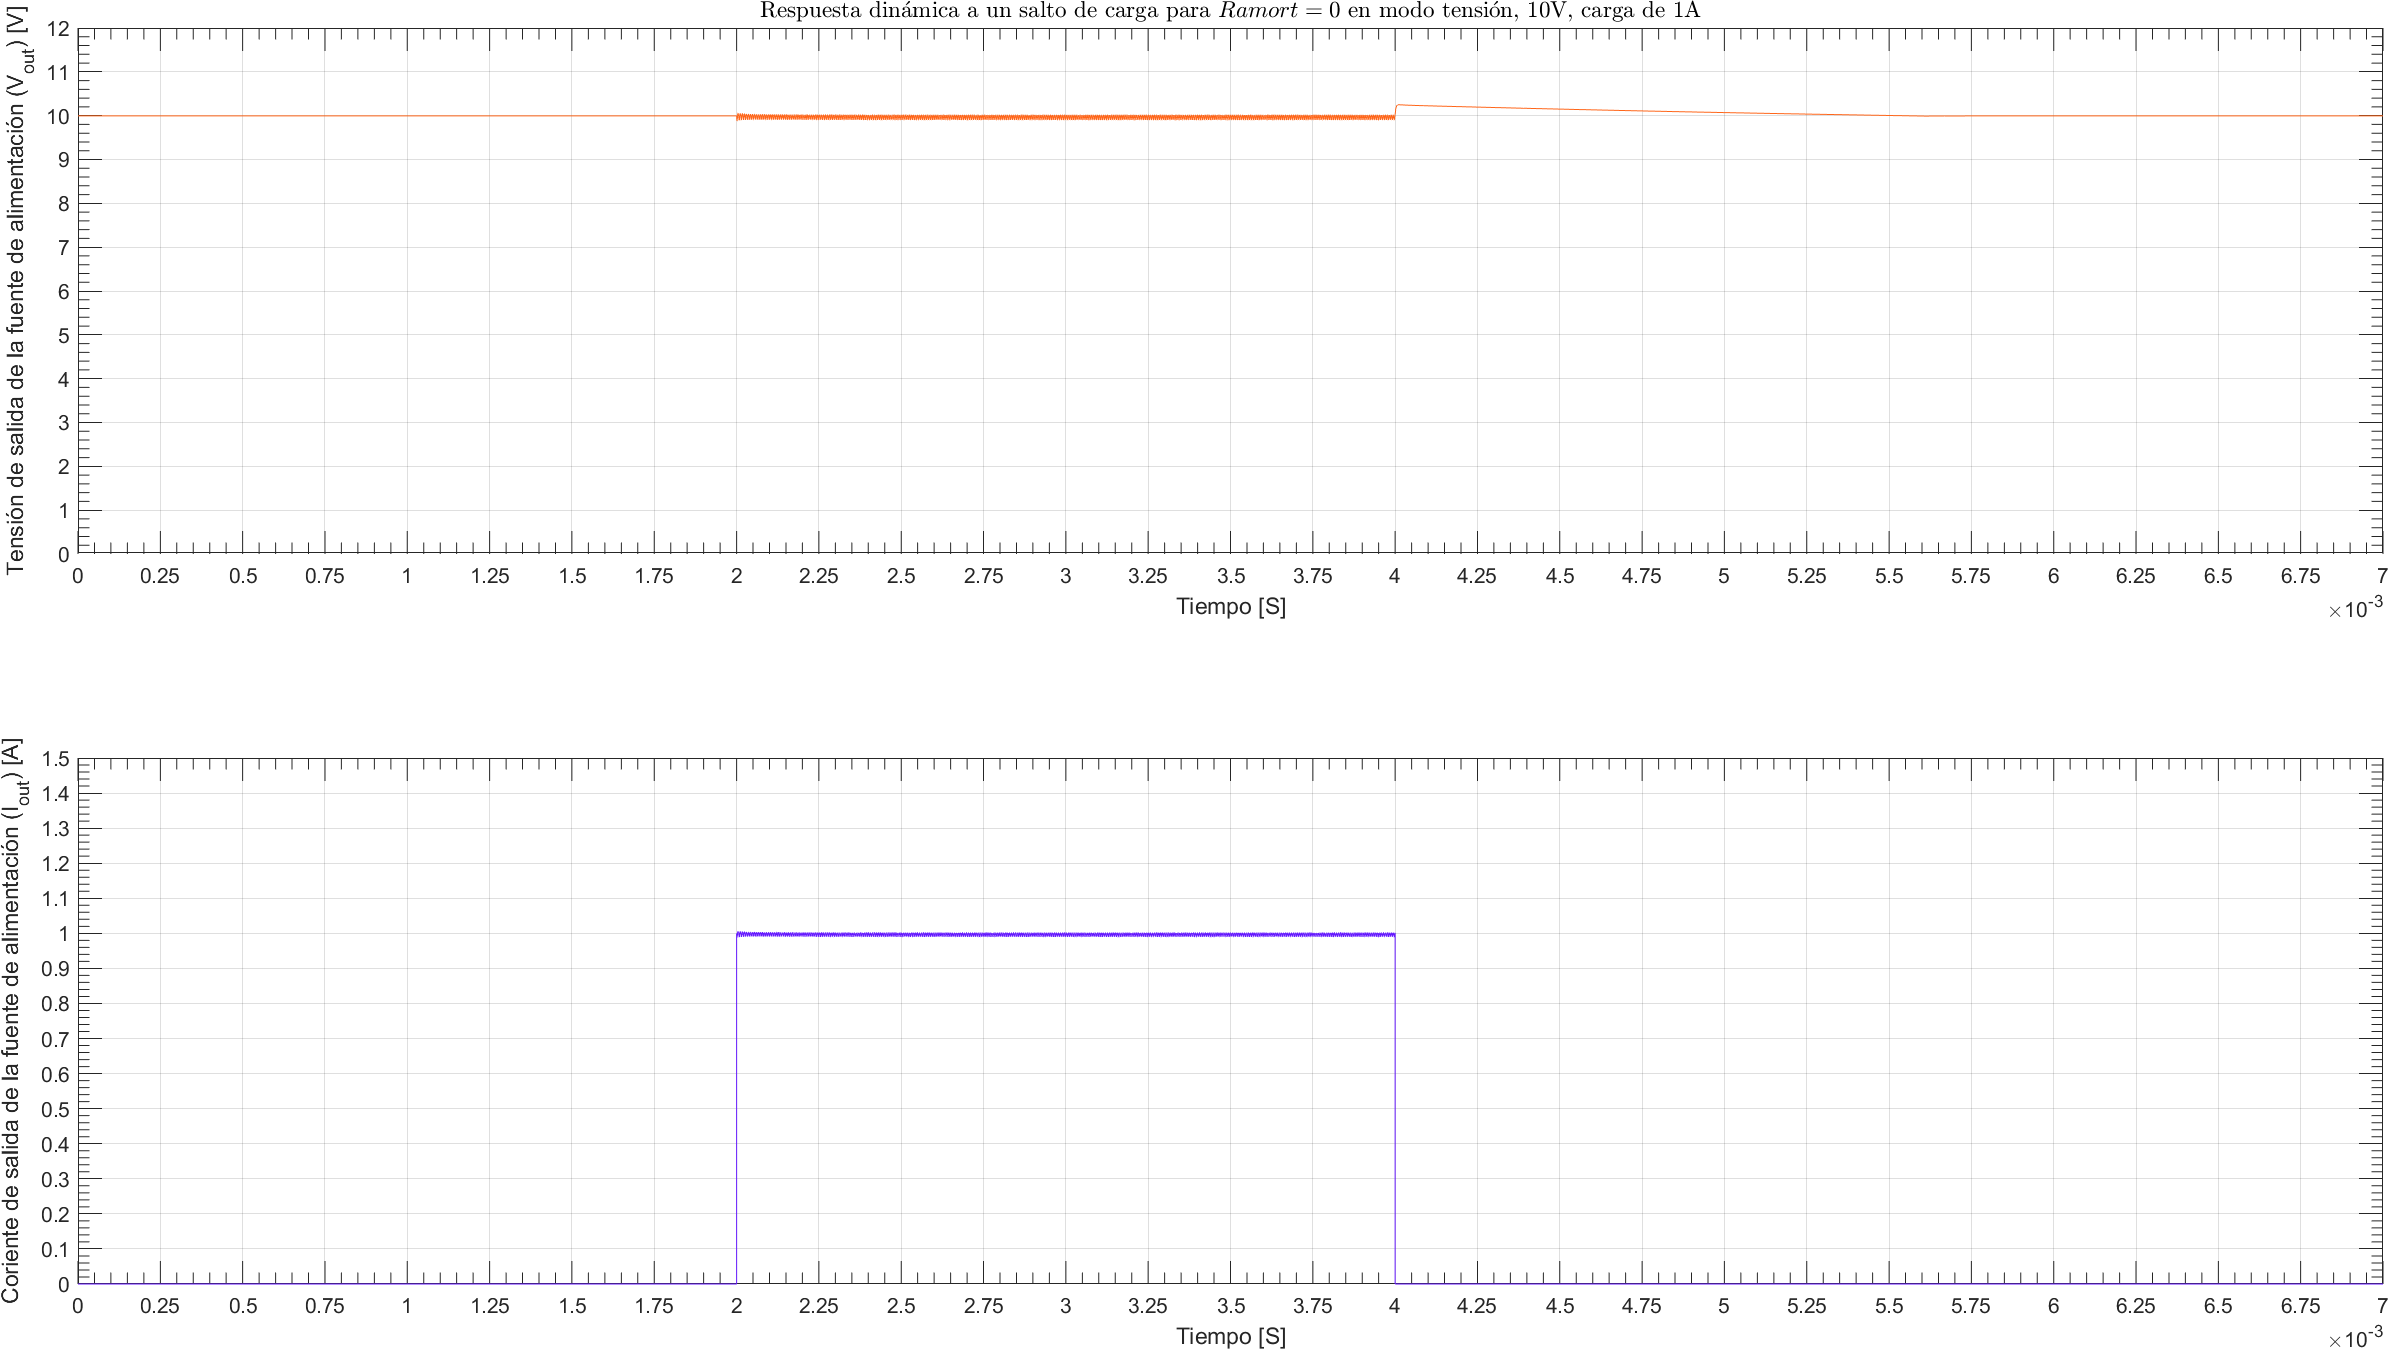
\includegraphics[width=1.1 \textwidth, angle=90]{./img/plots/dynamic/power_supply_RAMORT_0_STEP_Modo1.png}
\caption{\label{fig:fig_power_supply_RAMORT_STEP_0_Modo1}\footnotesize{Respuesta dinámica en modo tensión, $V_{out} = 10 \si[per-mode=symbol]{\volt}$, para $R_{amort} = 0 \si[per-mode=symbol]{\ohm} $.}}
\end{center}
\end{figure}

\clearpage

\begin{figure}[H] %htb
\begin{center}
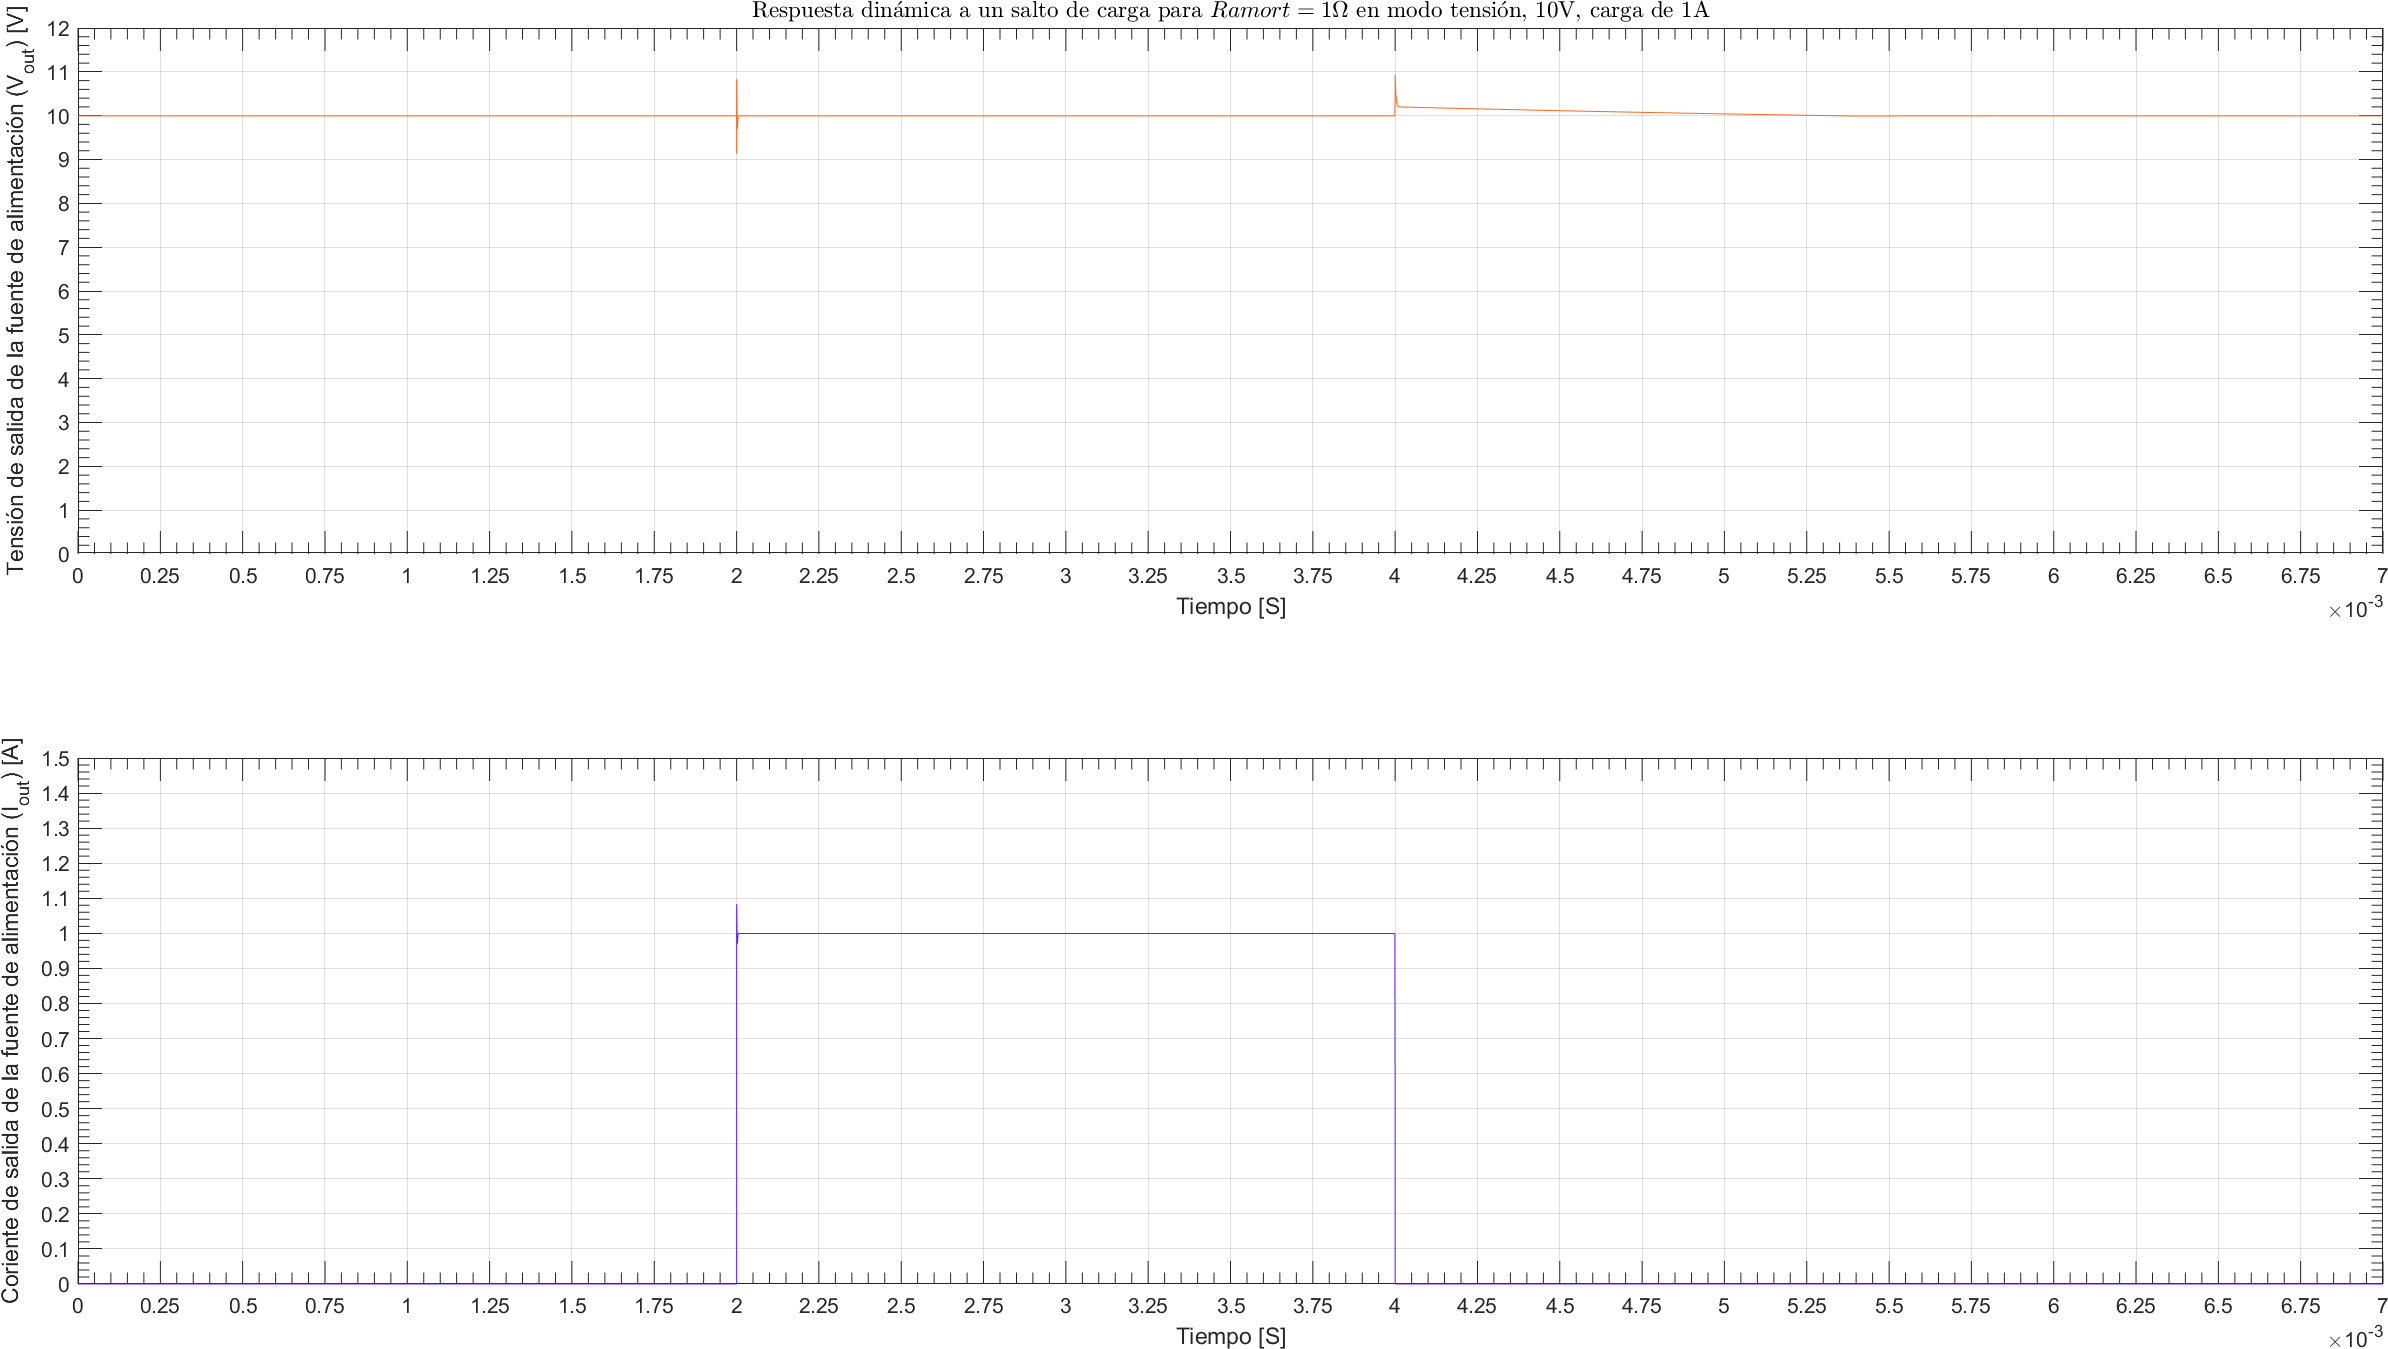
\includegraphics[width=1.1 \textwidth, angle=90]{./img/plots/dynamic/power_supply_RAMORT_1_STEP_Modo1.png}
\caption{\label{fig:fig_power_supply_RAMORT_STEP_1_Modo1}\footnotesize{Respuesta dinámica en modo tensión, $V_{out} = 10 \si[per-mode=symbol]{\volt}$, para $R_{amort} = 1 \si[per-mode=symbol]{\ohm} $.}}
\end{center}
\end{figure}

\clearpage

\begin{figure}[H] %htb
\begin{center}
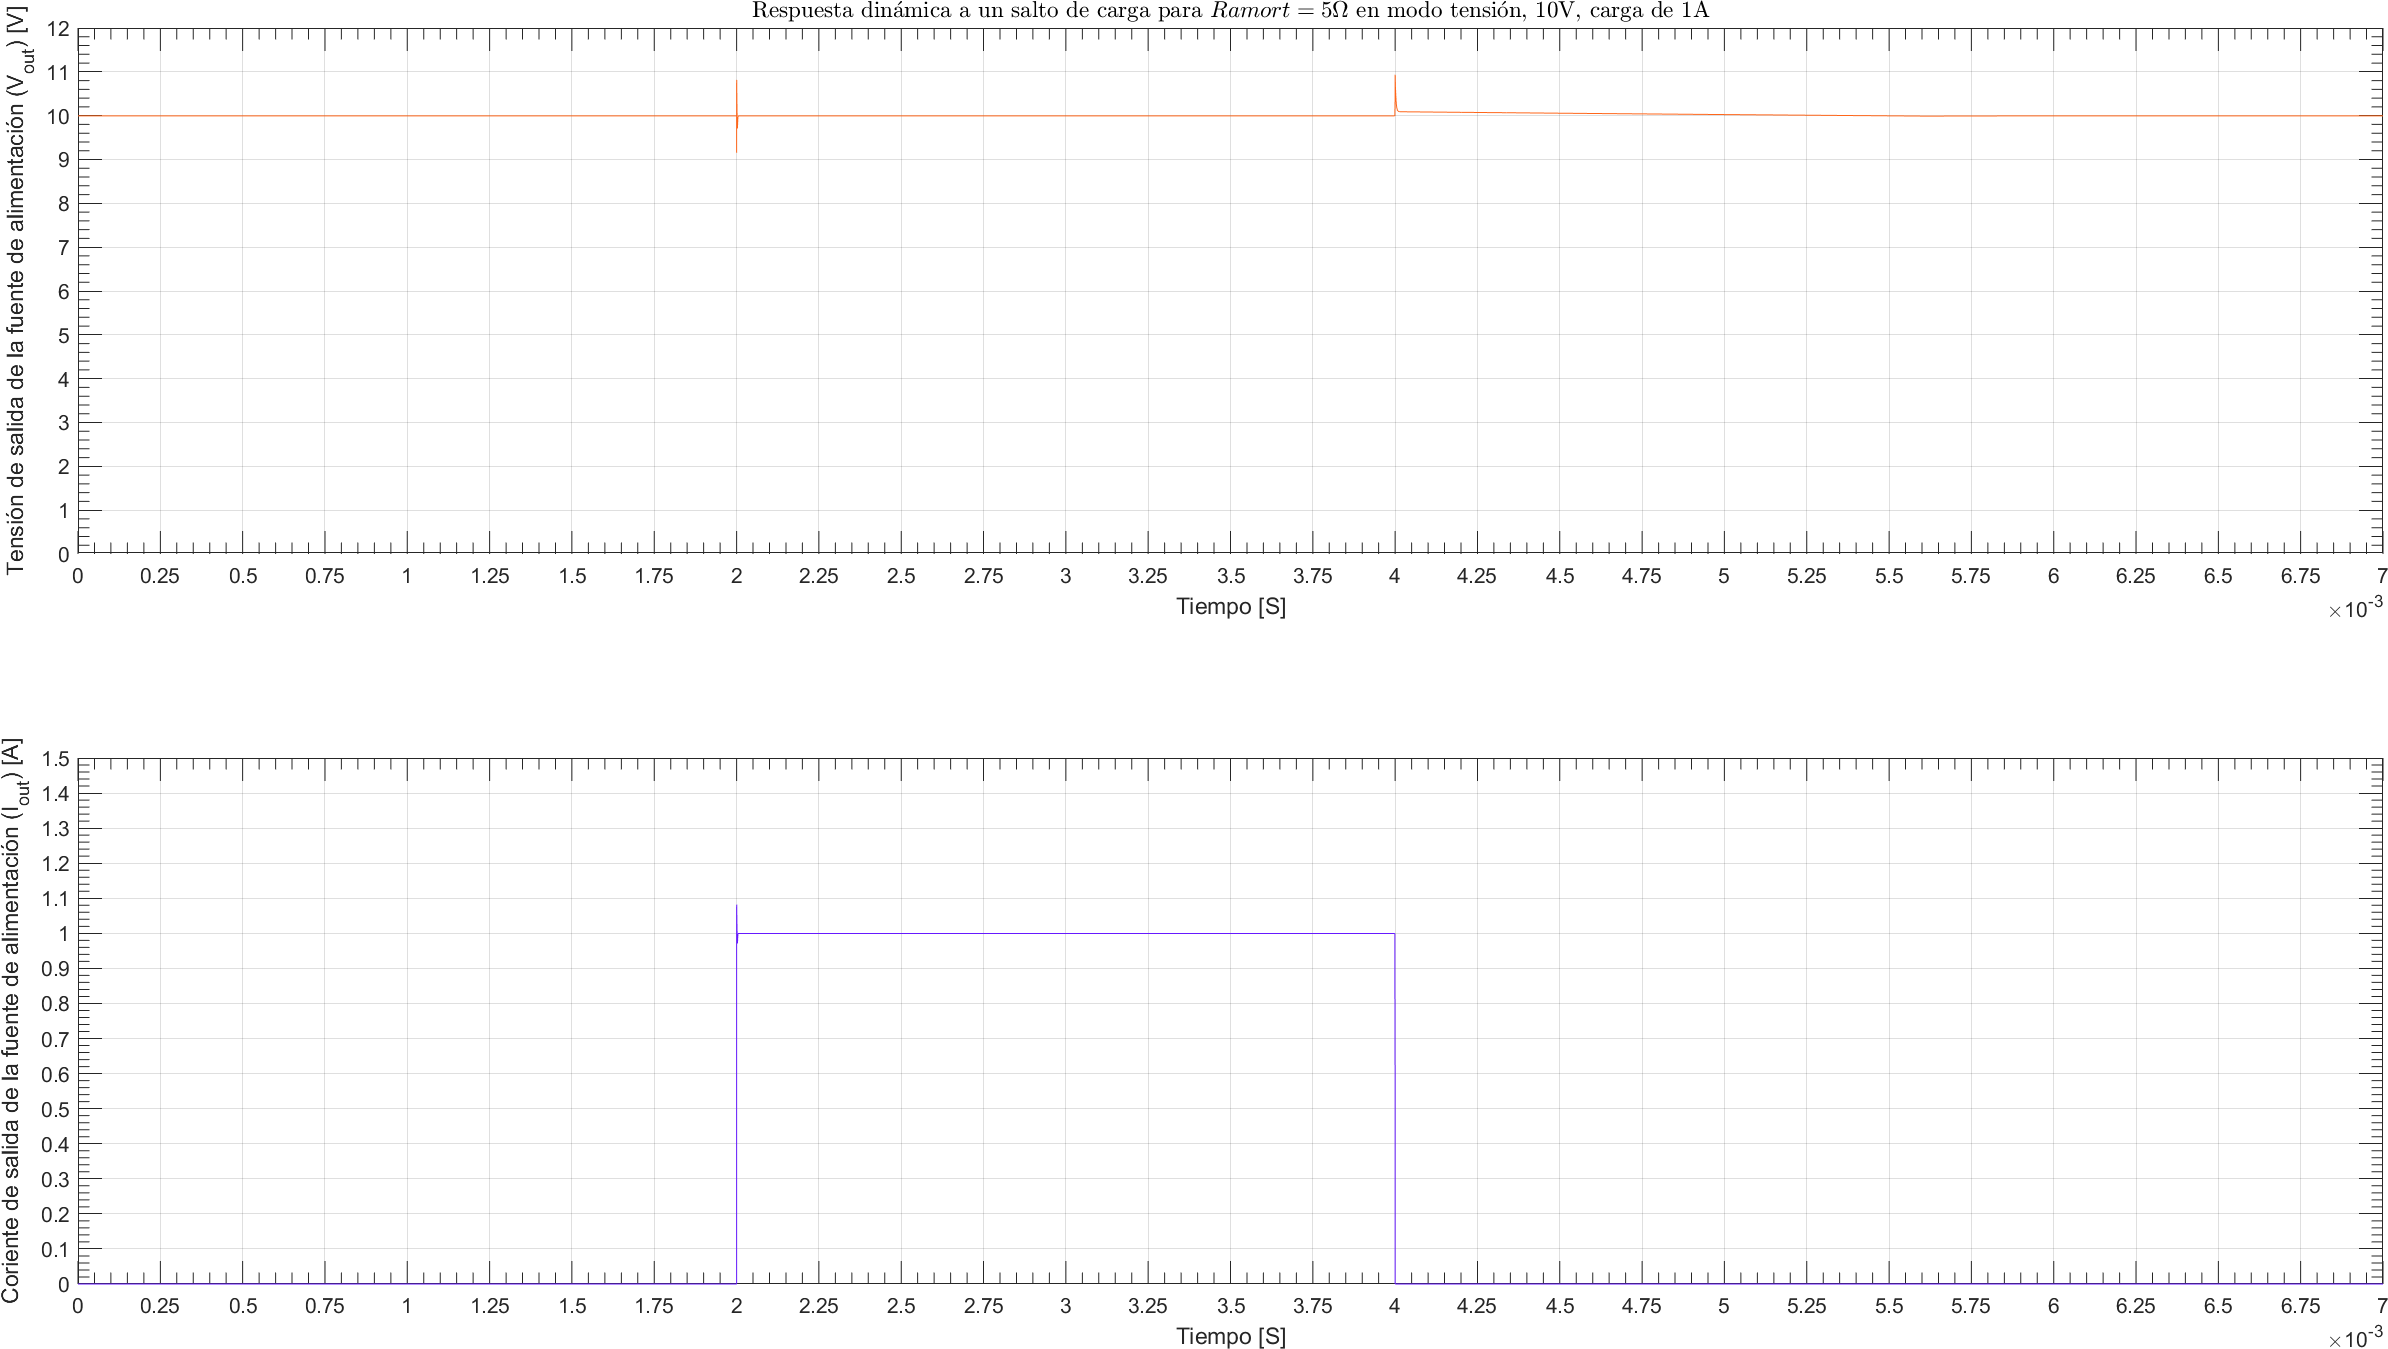
\includegraphics[width=1.1 \textwidth, angle=90]{./img/plots/dynamic/power_supply_RAMORT_5_STEP_Modo1.png}
\caption{\label{fig:fig_power_supply_RAMORT_STEP_5_Modo1}\footnotesize{Respuesta dinámica en modo tensión, $V_{out} = 10 \si[per-mode=symbol]{\volt}$, para $R_{amort} = 5 \si[per-mode=symbol]{\ohm} $.}}
\end{center}
\end{figure}

\clearpage


\subsubsection{Análisis para $R_{amort}$ en modo tensión, $V_{out} = 1 \si[per-mode=symbol]{\volt}$, $R_{L} = 1 \si[per-mode=symbol]{\ohm}$}

Se puede ver en la figura~\figref{fig:fig_power_supply_RAMORT_LOOP_Modo2} de ganancia de lazo para $R_{amort} = 0 \si[per-mode=symbol]{\ohm} $ que el margen de ganancia es $-0.5 \si[per-mode=symbol]{\decibel} $ y el margen de fase es $-1.4 \si[per-mode=symbol]{\degree} $ en condición de oscilación y en el gráfico de respuesta transitoria para $R_{amort} = 0 \si[per-mode=symbol]{\ohm} $, figura~\figref{fig:fig_power_supply_RAMORT_STEP_0_Modo2}, se ve como el sistema tiene una oscilación bastante marcada una vez que se alcanza la tensión del escalón y se mantiene hasta finalizar este, ya que no hay elemento disipativo, en cambio con $R_{amort} = 1 \si[per-mode=symbol]{\ohm} $, figura~\figref{fig:fig_power_supply_RAMORT_STEP_1_Modo2}, o $R_{amort} = 5 \si[per-mode=symbol]{\ohm} $, figura~\figref{fig:fig_power_supply_RAMORT_STEP_5_Modo2}, la respuesta transitoria ya no oscila, además se mejoran ampliamente los márgenes de fase y ganancia.

\vfill


% RAMORT MODO 2.

\clearpage

\begin{figure}[H] %htb
\begin{center}
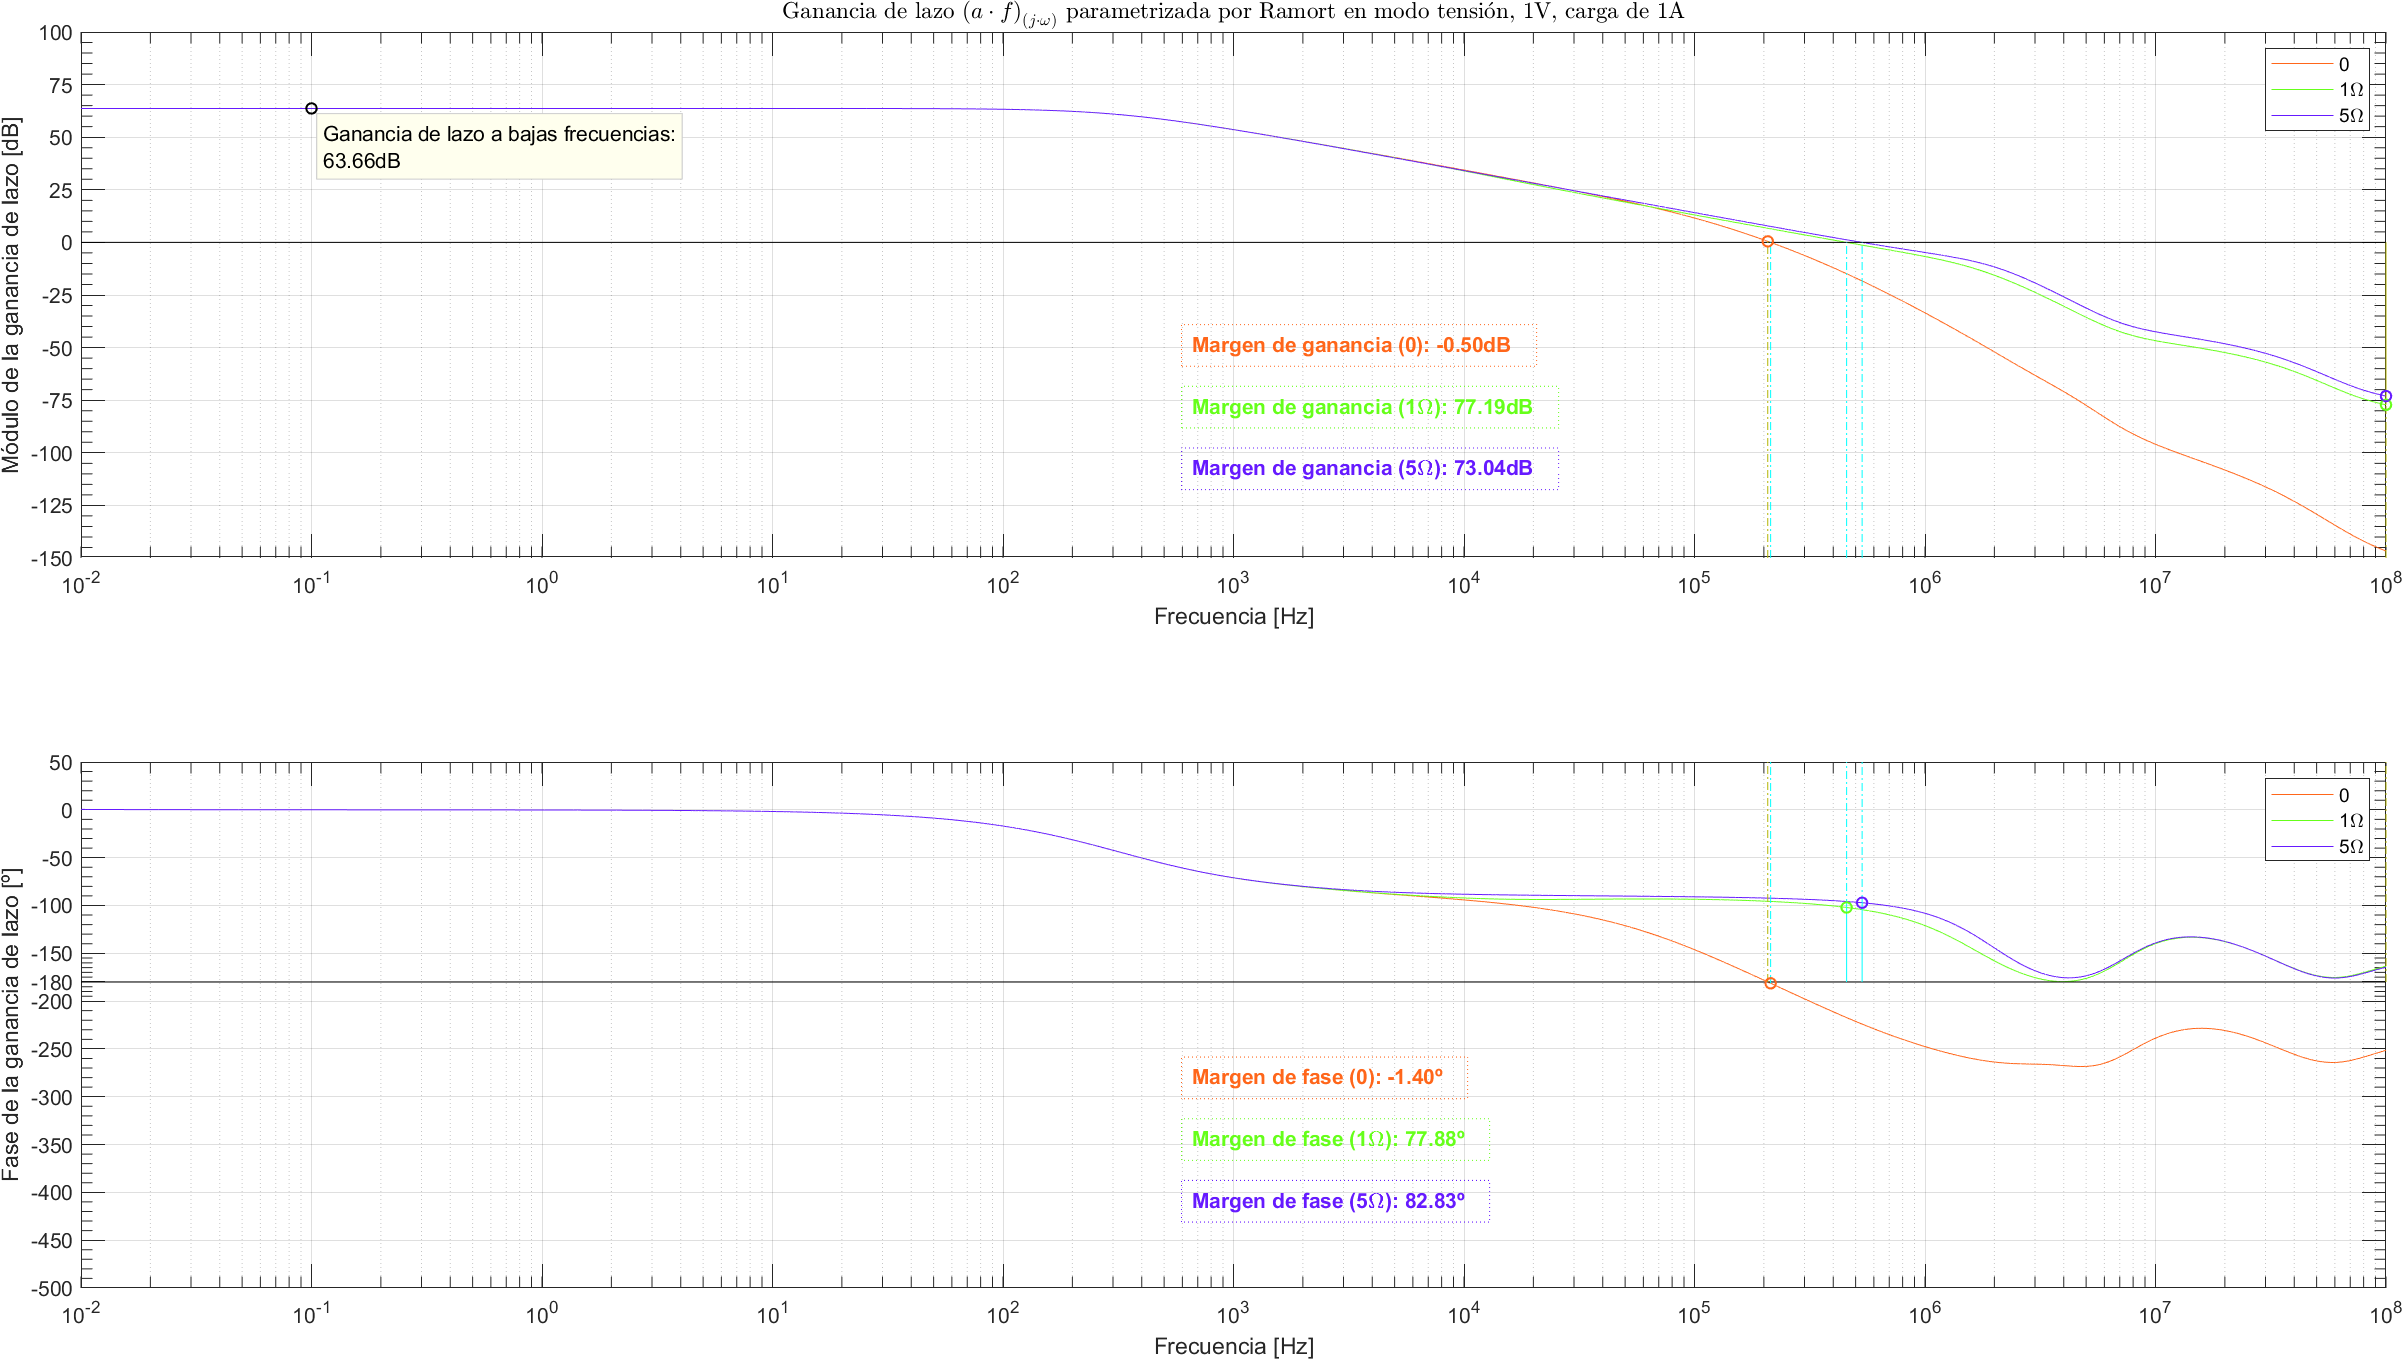
\includegraphics[width=1.1 \textwidth, angle=90]{./img/plots/loop/power_supply_RAMORT_LOOP_Modo2.png}
\caption{\label{fig:fig_power_supply_RAMORT_LOOP_Modo2}\footnotesize{Ganancia de lazo en modo tensión, $V_{out} = 1 \si[per-mode=symbol]{\volt}$, en función de la frecuencia parametrizada por $R_{amort}$.}}
\end{center}
\end{figure}


\clearpage

\begin{figure}[H] %htb
\begin{center}
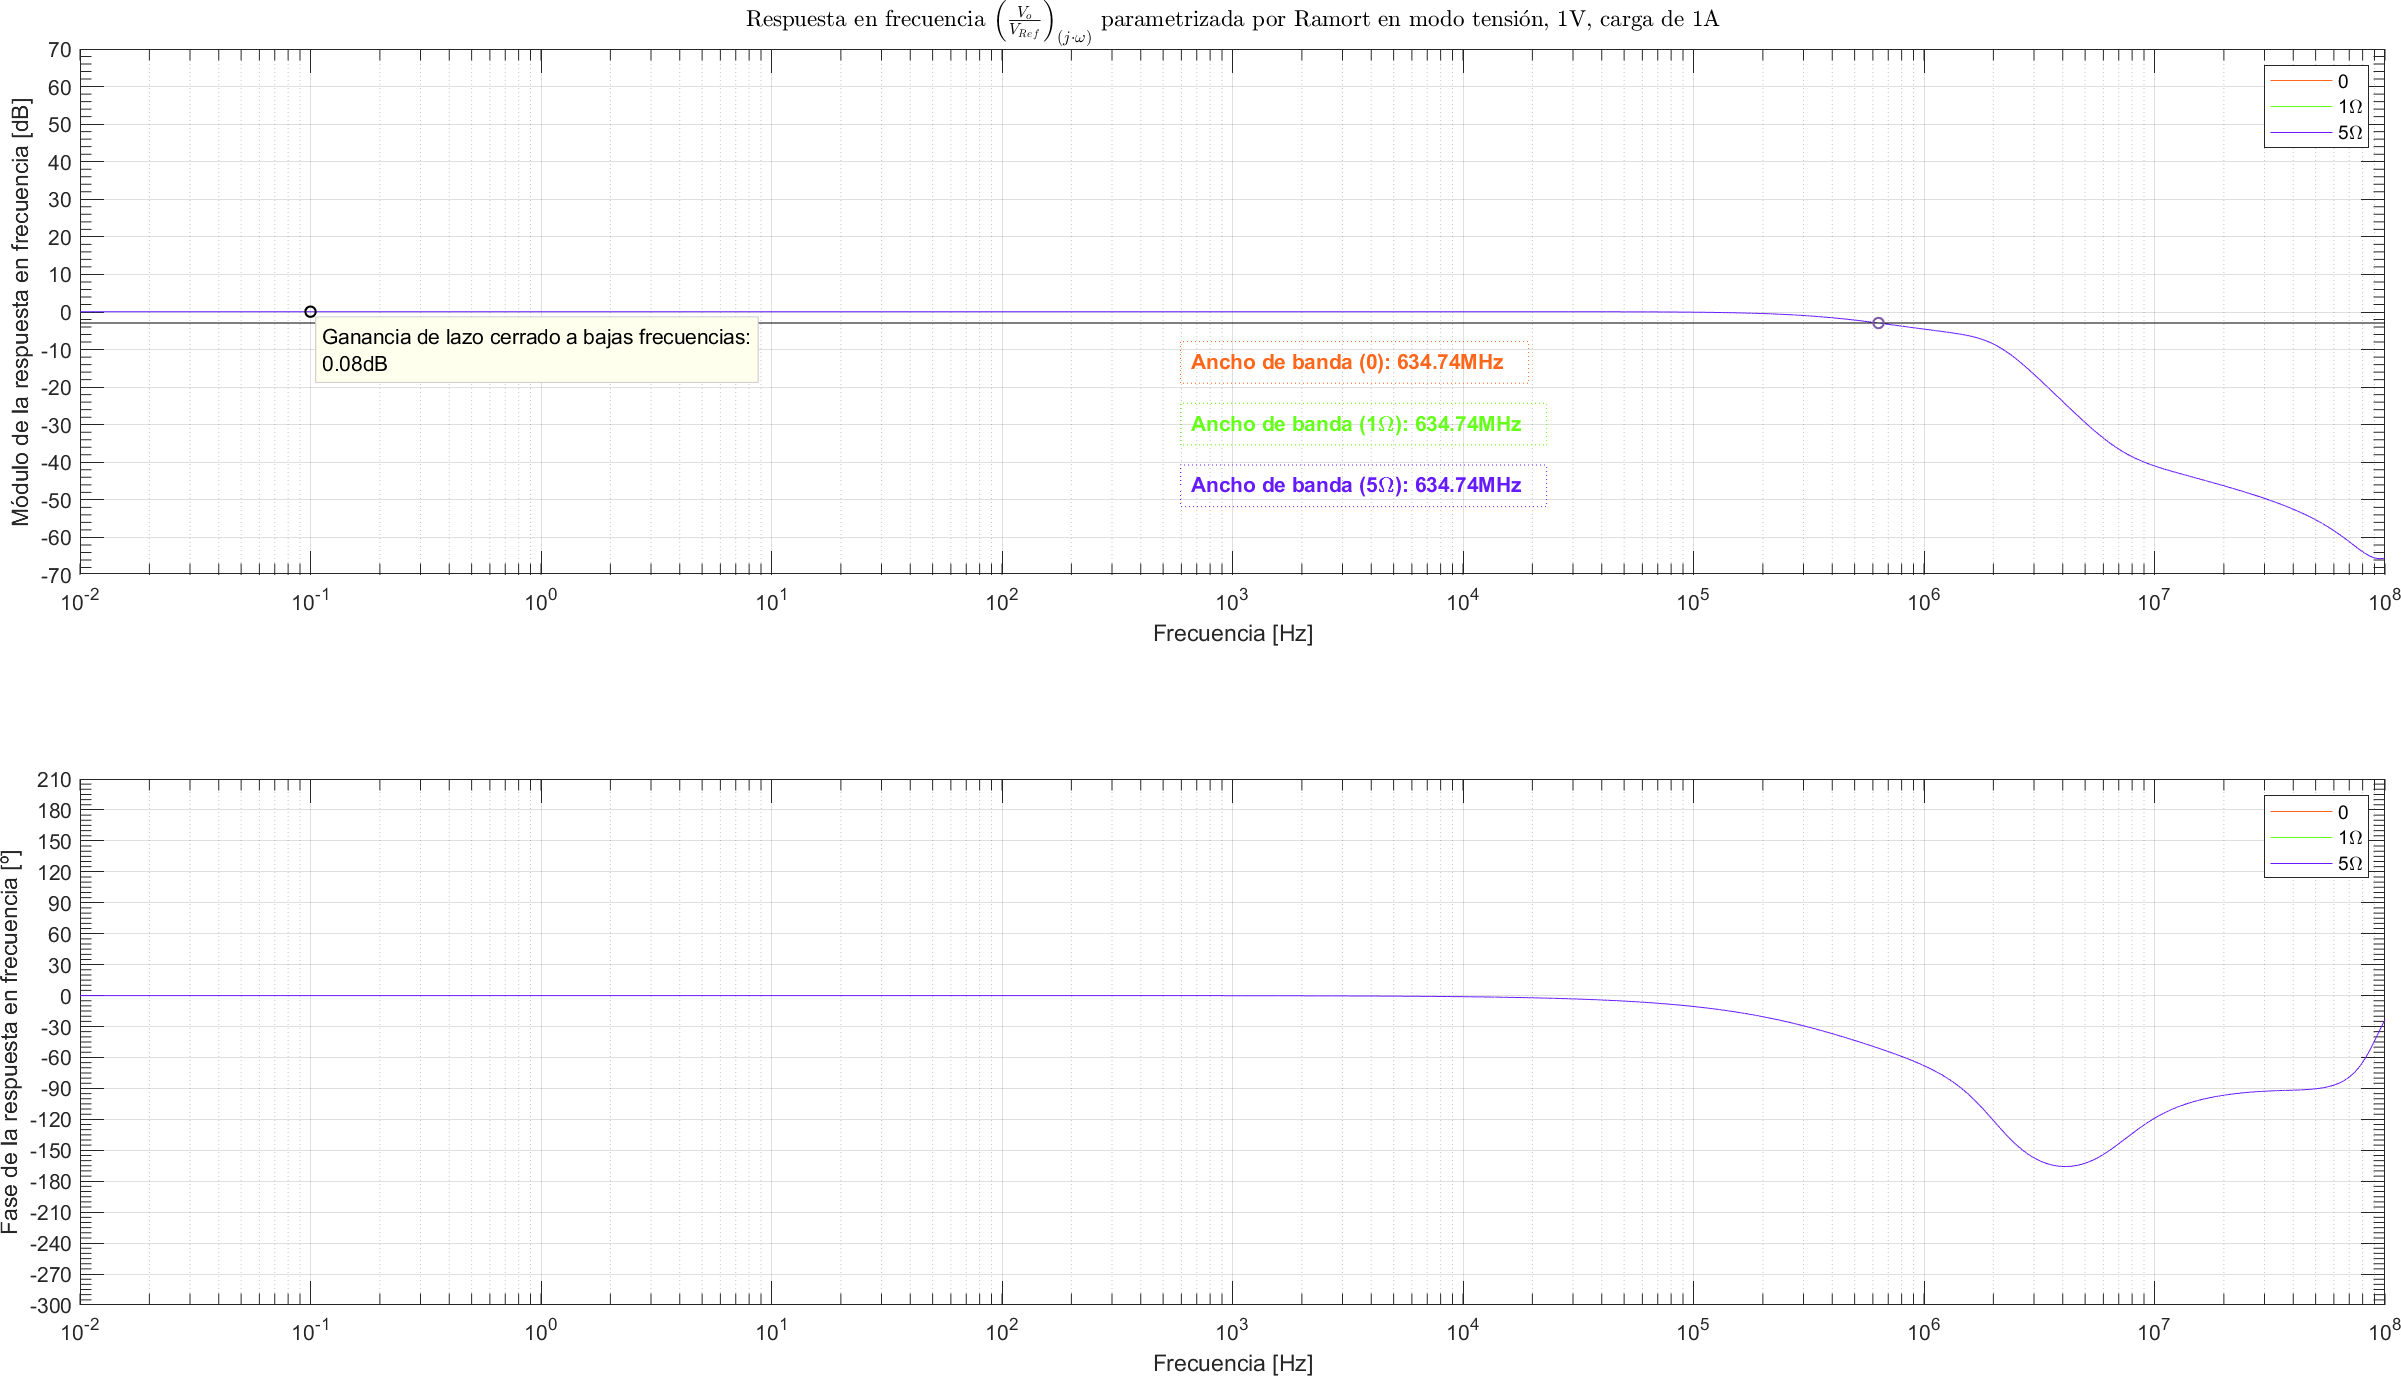
\includegraphics[width=1.1 \textwidth, angle=90]{./img/plots/rf/power_supply_RAMORT_RF_Modo2.png}
\caption{\label{fig:fig_power_supply_RAMORT_RF_Modo2}\footnotesize{Respuesta en frecuencia en modo tensión, $V_{out} = 1 \si[per-mode=symbol]{\volt}$, en función de la frecuencia parametrizada por $R_{amort}$.}}
\end{center}
\end{figure}

\clearpage

\begin{figure}[H] %htb
\begin{center}
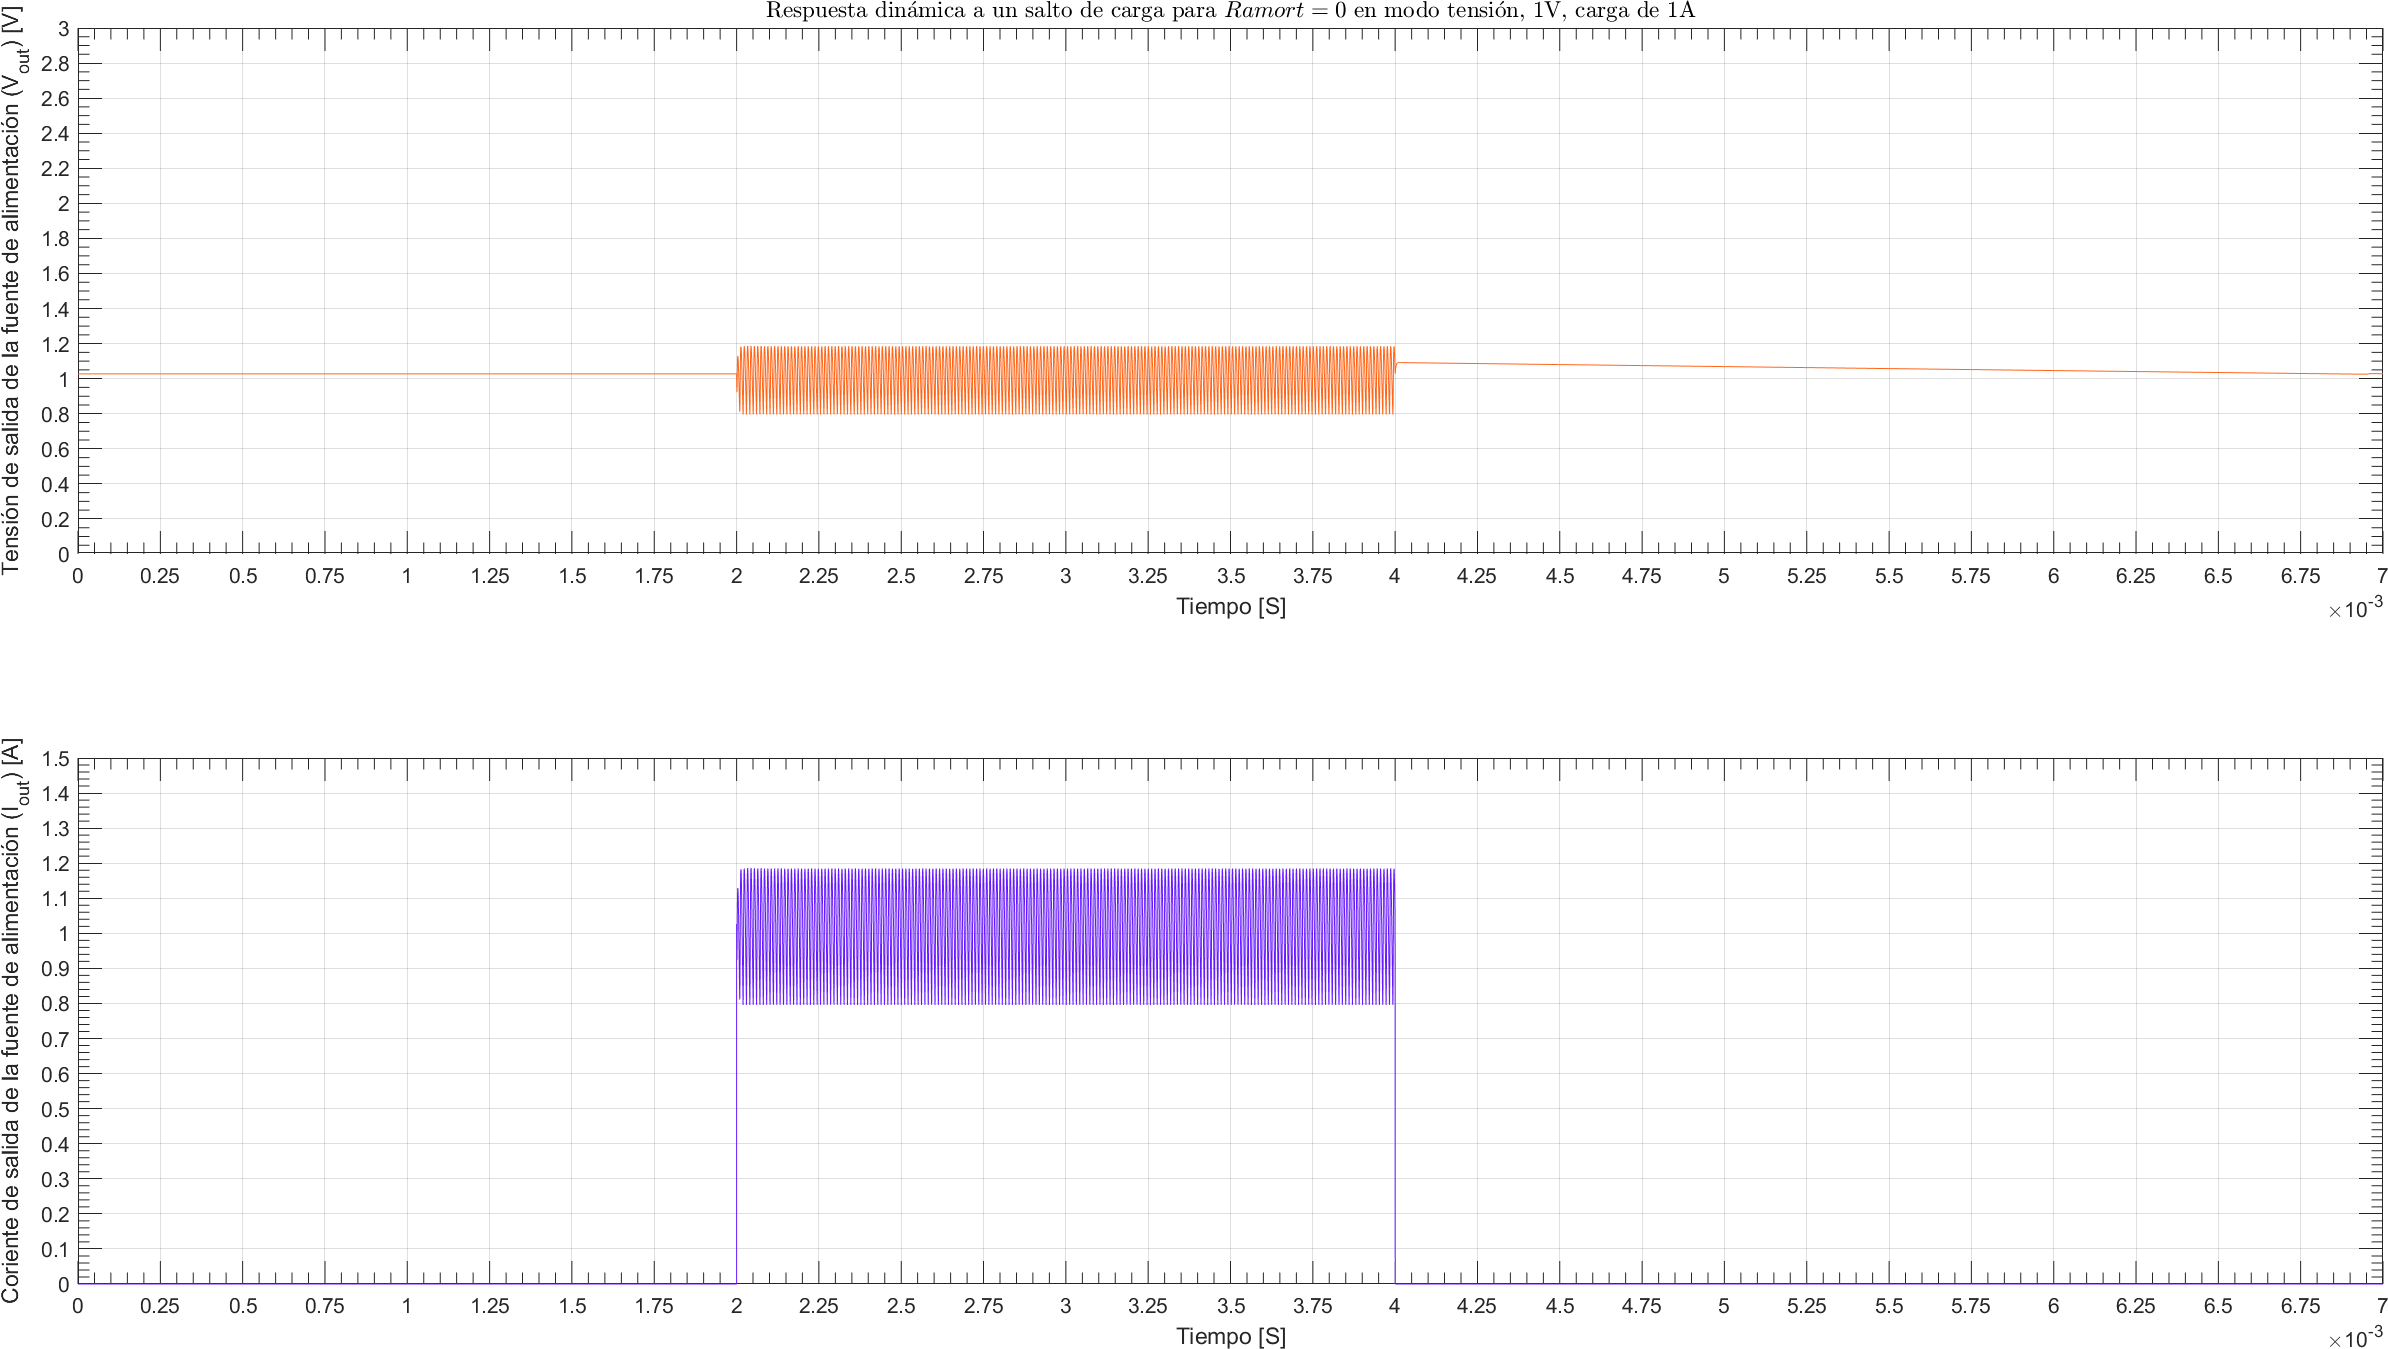
\includegraphics[width=1.1 \textwidth, angle=90]{./img/plots/dynamic/power_supply_RAMORT_0_STEP_Modo2.png}
\caption{\label{fig:fig_power_supply_RAMORT_STEP_0_Modo2}\footnotesize{Respuesta dinámica en modo tensión, $V_{out} = 1 \si[per-mode=symbol]{\volt}$, para $R_{amort} = 0 \si[per-mode=symbol]{\ohm} $.}}
\end{center}
\end{figure}

\clearpage

\begin{figure}[H] %htb
\begin{center}
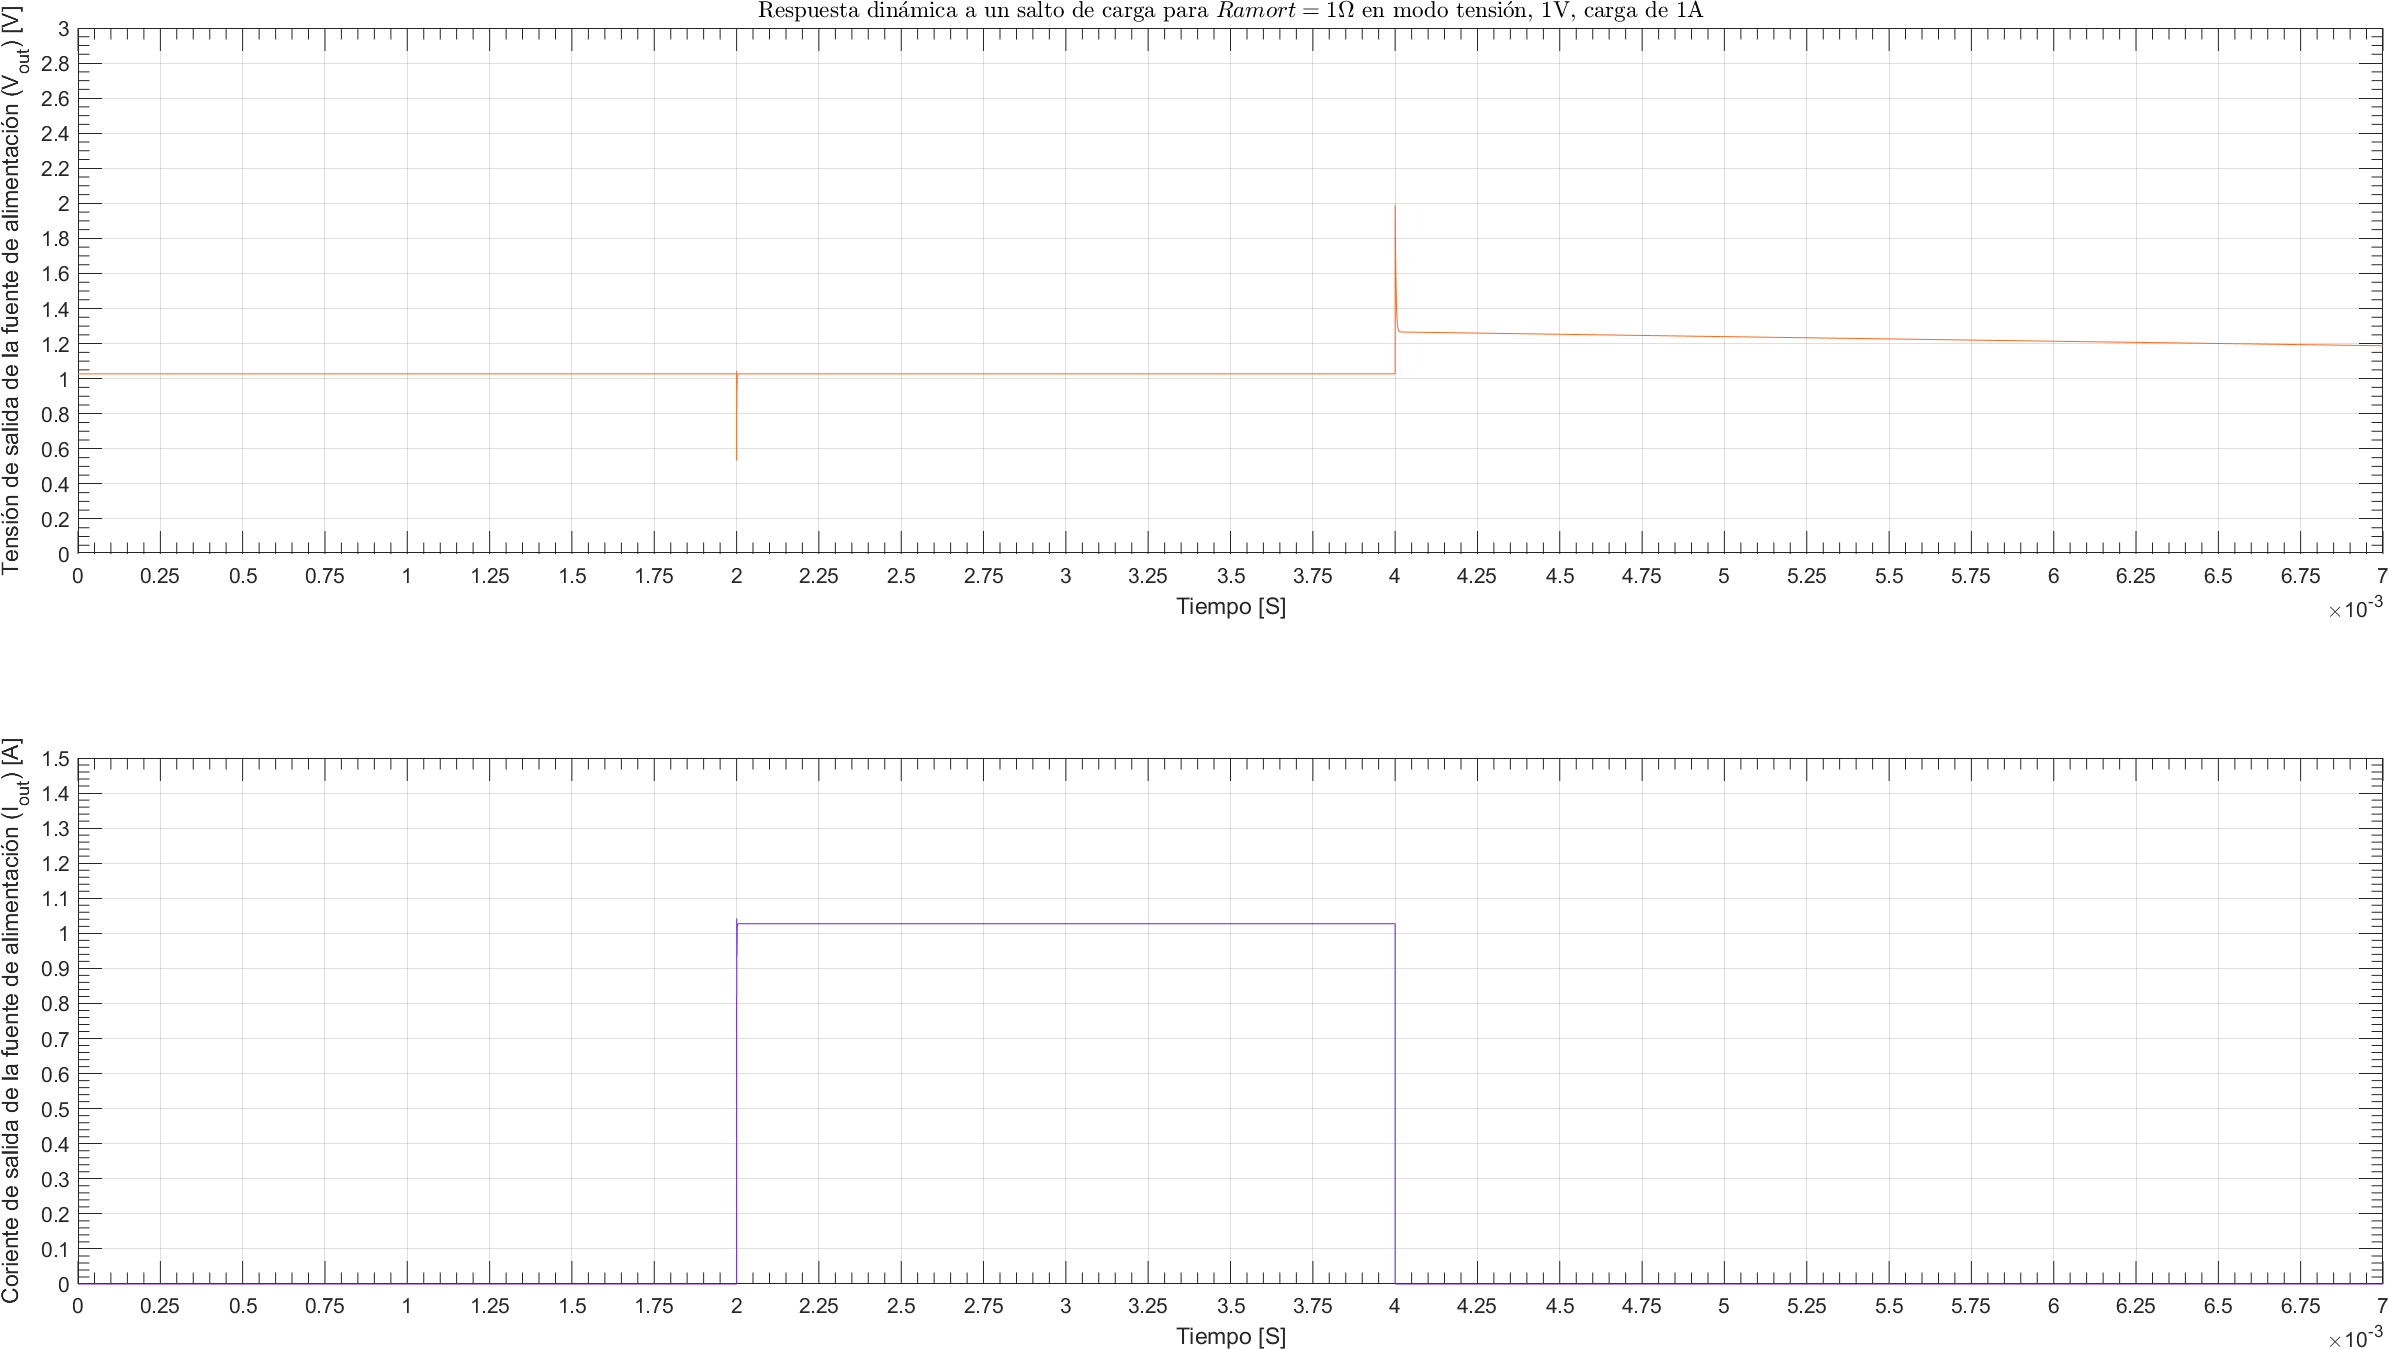
\includegraphics[width=1.1 \textwidth, angle=90]{./img/plots/dynamic/power_supply_RAMORT_1_STEP_Modo2.png}
\caption{\label{fig:fig_power_supply_RAMORT_STEP_1_Modo2}\footnotesize{Respuesta dinámica en modo tensión, $V_{out} = 1 \si[per-mode=symbol]{\volt}$, para $R_{amort} = 1 \si[per-mode=symbol]{\ohm} $.}}
\end{center}
\end{figure}

\clearpage

\begin{figure}[H] %htb
\begin{center}
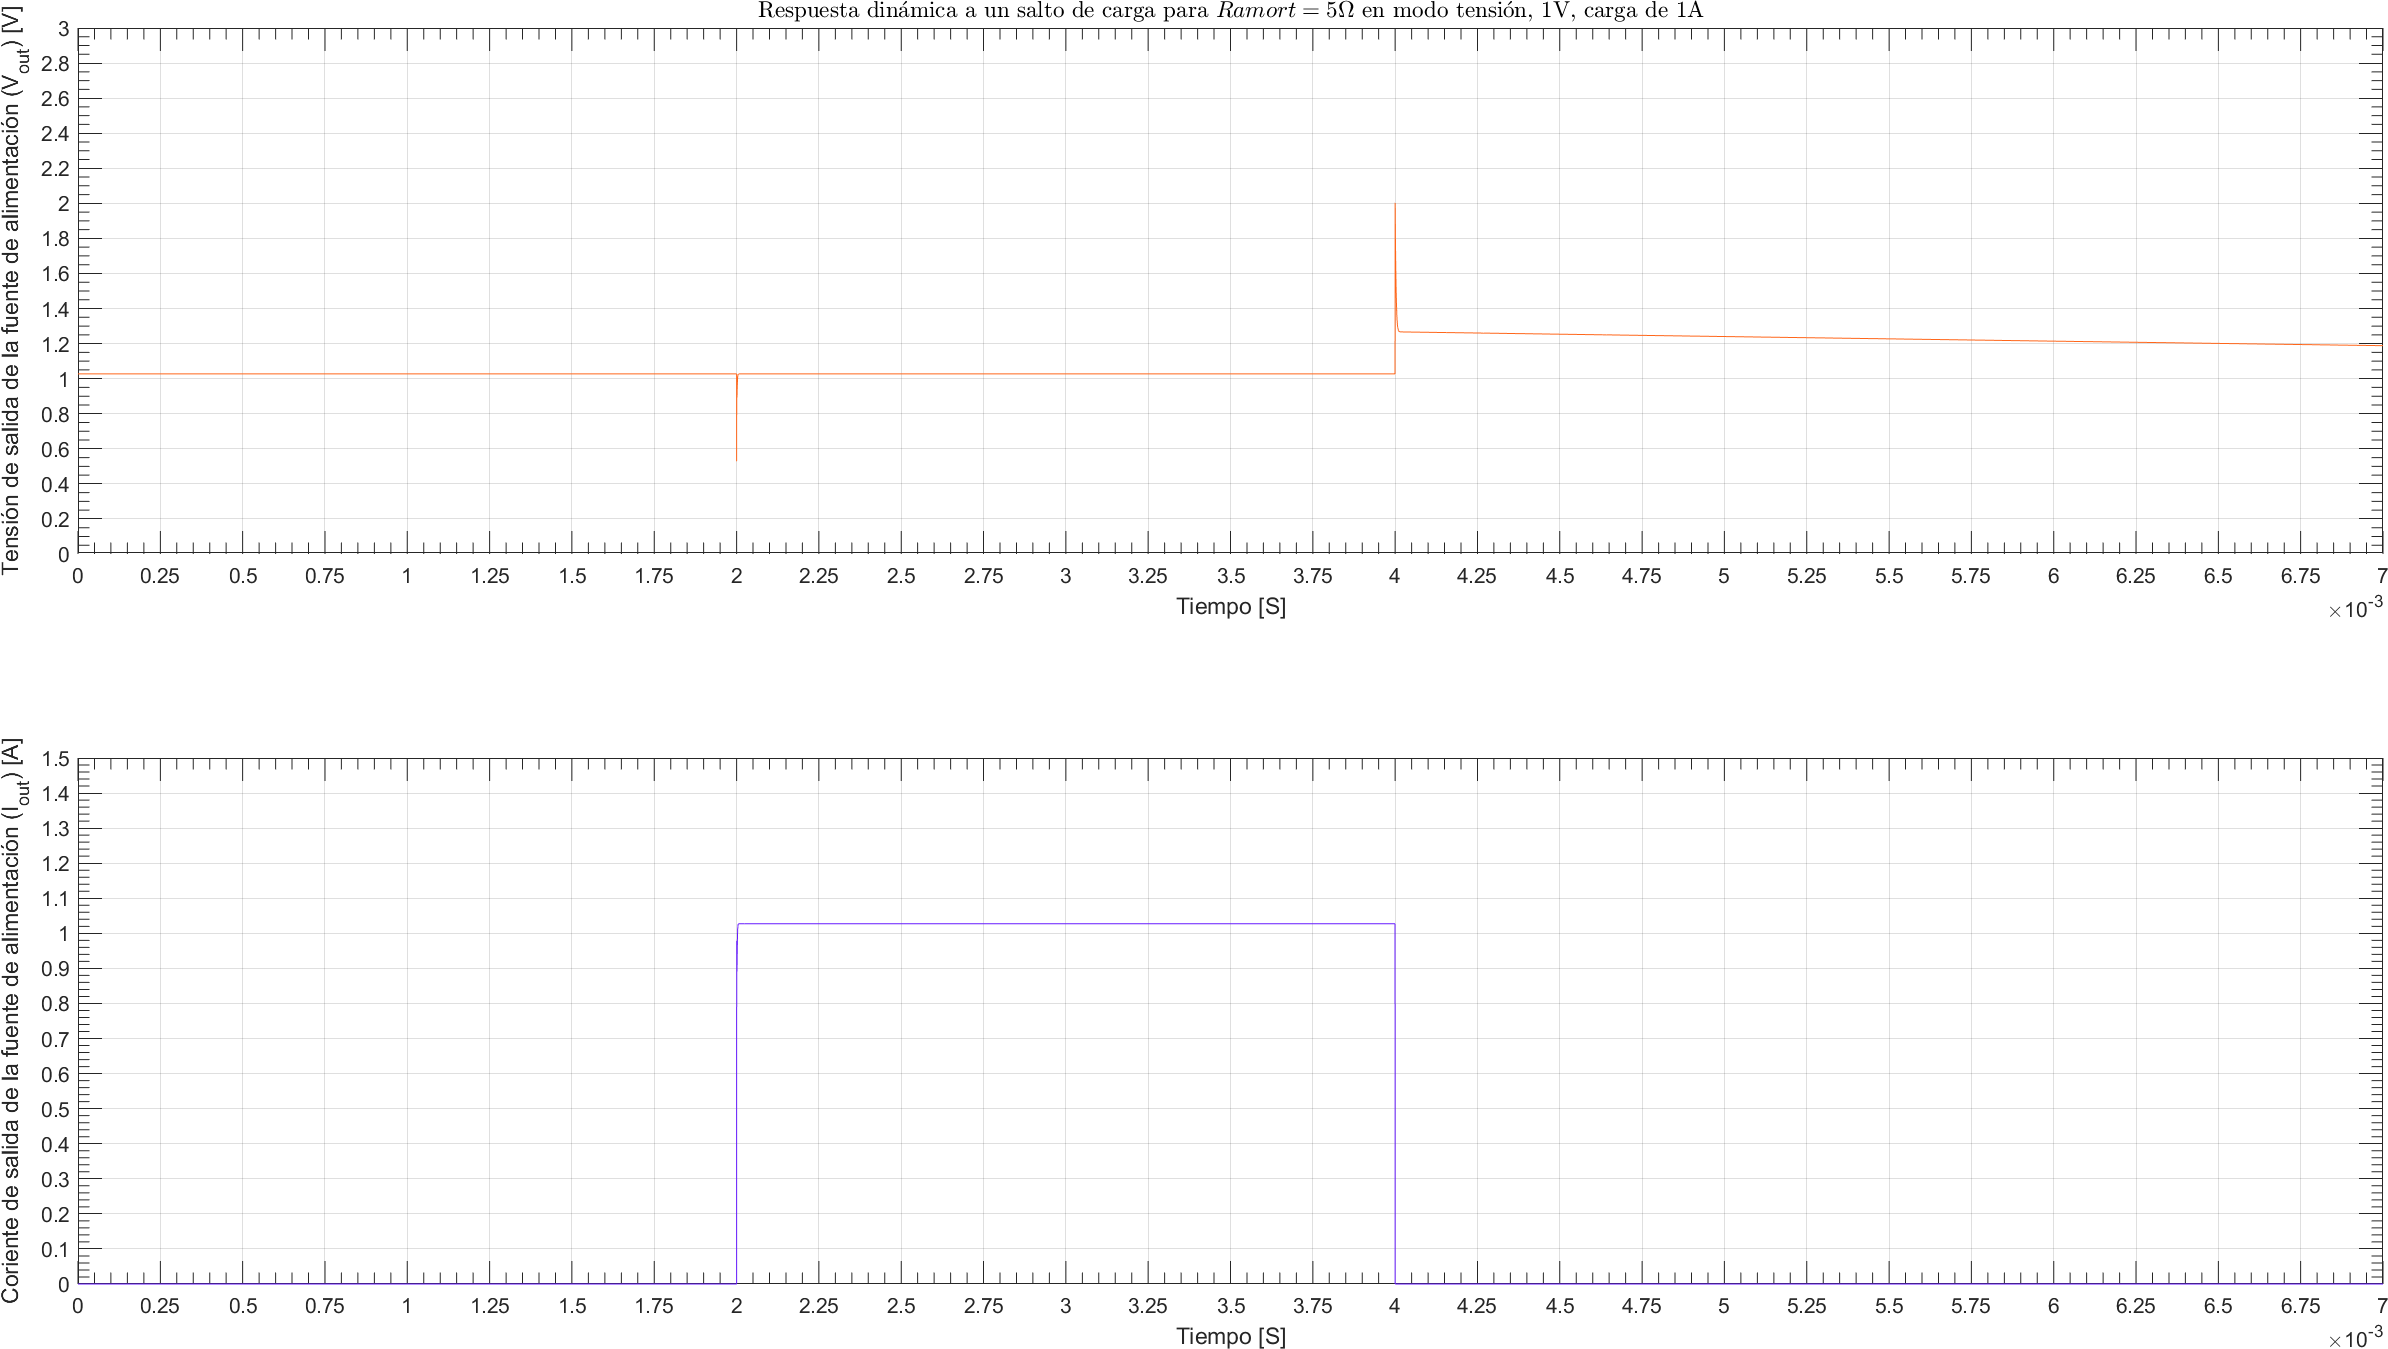
\includegraphics[width=1.1 \textwidth, angle=90]{./img/plots/dynamic/power_supply_RAMORT_5_STEP_Modo2.png}
\caption{\label{fig:fig_power_supply_RAMORT_STEP_5_Modo2}\footnotesize{Respuesta dinámica en modo tensión, $V_{out} = 1 \si[per-mode=symbol]{\volt}$, para $R_{amort} = 5 \si[per-mode=symbol]{\ohm} $.}}
\end{center}
\end{figure}

\clearpage
